
\documentclass[10pt, conference, compsocconf]{IEEEtran}

% ICTAI 2015: max 8 pages

% correct bad hyphenation here
\hyphenation{op-tical net-works semi-conduc-tor}
\usepackage{algorithm}
\usepackage{algorithmic}
\usepackage{pstricks,graphicx}
\usepackage{amsmath,amssymb,amsfonts}

\newcommand{\rr}{{\mathbf{r}}}
\newcommand{\vv}{{\mathbf{v}}}
\newcommand{\xx}{{\mathbf{x}}}
\newcommand{\yy}{{\mathbf{y}}}
\newcommand{\Matrix}[1]{\mathsf{#1}}
\newcommand{\mat}[1]{\Matrix{#1}}
\newcommand{\transpose}{^\mathsf{T}}
\newcommand{\sgn}{\text{sgn}}
\newcommand{\mm}{{\boldsymbol{{\mu}}}}
\newcommand{\celsius}{$^{\circ}$C}

\newcommand{\refeq}[1]{(\ref{eq:#1})}
\newcommand{\reffig}[1]{fig.~\ref{fig:#1}}
\newcommand{\refFig}[1]{Fig.~\ref{fig:#1}}
\newcommand{\reftab}[1]{table~\ref{tab:#1}}
\newcommand{\refTab}[1]{Table~\ref{tab:#1}}
\newcommand{\refsection}[1]{section~\ref{sec:#1}}
\newcommand{\refSection}[1]{Section~\ref{sec:#1}}
\newcommand{\refAppendix}[1]{Appendix~\ref{appendix:#1}}
\newcommand{\refappendix}[1]{appendix~\ref{appendix:#1}}


\newcommand{\unitone}[1]{\left[\text{#1}\right]}
\newcommand{\unittwo}[2]{\left[\frac{\text{#1}}{\text{#2}}\right]}


\begin{document}
%
% can use linebreaks \\ within to get better formatting as desired
\title{Original CSTR}

\maketitle


\section{Continuous Stirred Tank Reactor (CSTR)}\label{sec:CSTR}

The object of study is a sophisticated simulator of a
jacketed chemical reactor where an exothermic reaction takes place,
shown in \reffig{CSTR_model}. It was used as a benchmark for an
expert system like diagnosis environment in two doctoral theses
in Chemical Engineering at the Massachusetts Institute of Technology
\cite{phdthesisFinch1989}, \cite{phdthesisOyeleye1990},
from now called the MIT-CSTR. 
The motivation to use this process is its high non-linearity,
that it has interacting control loops, that it has multiple causal
pathways with opposing tendencies between variables, thus making the
process an appropriate candidate for causal analysis.
Another aspect of the CSTR process is the complete availability
of its analytic description. The highly popular
Tennessee-Eastman (TE) chemical process \cite{downs1993plant,chiang2001fault},
is frequently used as the
experimental benchmark for complex data-driven
process condition detection techniques
\cite{Rato2013101,Chen201433,Askarian2016104,Yin2012comparison,Yin2014realtime}.
However, it deliberately lacks the underlying description
of the mass and heat balances, the control algorithms
and the simulation framework. The TE source code is available,
however in an obfuscated way. On the other hand, the complete transparency
of the MIT-CSTR allows the researcher a deeper understanding
of the process dynamics, leading to more consolidated affirmations
about his fault diagnosis methods.
\begin{figure*}[htb!]
\centering
\definecolor{grey95}{rgb}{0.98,0.98,0.98}

\newcommand{\ts}[1]{\text{\scriptsize{#1}}}
\newcommand{\tsi}[2]{\text{\scriptsize{#1}$_{#2}$}}
%\newcommand{\tsi}[2]{\text{\scriptsize{#1}}$_{\text{\tiny{#2}}}$}


\newcommand{\bal}[1]{\pscircle[fillstyle=solid,fillcolor=white](0.28,0.08){0.38}{#1}}
\newcommand{\bala}[1]{\pscircle[fillstyle=solid,fillcolor=white](0.12,0.10){0.3}{#1}}
\newcommand{\balb}[1]{\pscircle[fillstyle=solid,fillcolor=white](0.22,0.09){0.34}{#1}}
\newcommand{\balc}[1]{\pscircle[linewidth=0.5pt,linestyle=dashed,dash=2pt 1pt,
	fillstyle=solid,fillcolor=white](0.16,0.10){0.3}{#1}}
\newcommand{\bald}[1]{\pscircle[linewidth=0.5pt,linestyle=dashed,dash=2pt 1pt,
	fillstyle=solid,fillcolor=white](0.32,0.06){0.38}{#1}}
\newcommand{\bale}[1]{\pscircle[fillstyle=solid,fillcolor=white](0.07,0.08){0.25}{\scriptsize{#1}}}
\newcommand{\balf}[1]{\pscircle[fillstyle=solid,fillcolor=white](0.12,0.08){0.25}{\scriptsize{#1}}}

%\newcommand{\head}[1]{\psellipse[dimen=inner,fillstyle=none]
%	(0.5,0.1)(0.66,0.36){#1}}
\newcommand{\headpos}[1]{\pspolygon[linewidth=0.25pt,linestyle=dashed,dash=2pt 1pt,
	dimen=inner,fillstyle=solid,fillcolor=grey95](-0.1,-0.30)(-0.1,0.50)(1.2,0.35)(1.2,-0.15){#1}} % e.g. valve
	
\newcommand{\headneg}[1]{\pspolygon[linewidth=0.25pt,linestyle=dashed,dash=2pt 1pt,
	dimen=inner,fillstyle=solid,fillcolor=grey95](-0.1,0.28)(-0.1,-0.05)(1.2,-0.15)(1.2,0.40){#1}} % e.g. pump


\newpsstyle{arrstylepipe}{linewidth=1.5pt,showpoints=false,
        arrows=->,arrowsize=5.0pt 0,arrowlength=2.0,arrowinset=0}
\newpsobject{pipe}{psline}{style=arrstylepipe}

\newpsstyle{arrstylecontrol}{linewidth=1.0pt,showpoints=false,
        arrows=->,arrowsize=3.0pt 0,arrowlength=1.5,arrowinset=0}
\newpsobject{setpoint}{psline}{style=arrstylecontrol}

\newpsstyle{sensorstyle}{linewidth=1.0pt,showpoints=false}
\newpsobject{sensor}{psline}{style=sensorstyle}
\newpsstyle{sensorstyledashed}{linewidth=1.0pt,showpoints=false,linestyle=dashed,dash=2pt 1pt}
\newpsobject{sensordashed}{psline}{style=sensorstyledashed}


%%% VALVE
\newcommand{\valve}[0]{
		\pspolygon[linewidth=1pt,fillstyle=solid,fillcolor=white]
			(-0.18,-0.18)(0.18,0.18)(-0.18,0.18)(0.18,-0.18)
		\psline[linewidth=2pt](0,0)(0.30,0)
		\pswedge[dimen=inner,fillstyle=solid,fillcolor=white](0.30,0){0.18}{-90}{90}
}
%%% RESISTANCE
\newcommand{\resistance}[0]{\pspolygon[linewidth=1pt,fillstyle=solid,fillcolor=black]
	(-0.18,-0.18)(0.18,0.18)(-0.18,0.18)(0.18,-0.18)}
\newcommand{\resistancesmall}[0]{\pspolygon[linewidth=1pt,fillstyle=solid,fillcolor=black]
	(-0.12,-0.12)(0.12,0.12)(-0.12,0.12)(0.12,-0.12)}
%%% PUMP
\newcommand{\pump}[0]{
	\pspolygon[linewidth=1.0pt,fillstyle=solid,fillcolor=white](-0.35,-0.5)(0,0)(0.35,-0.5)
	\pscircle[linewidth=1.0pt,fillstyle=solid,fillcolor=white](0,0){0.35}
}
%%% PID CONTROLLER
\newcommand{\pid}[1]{\psframe[dimen=middle,linewidth=0.5pt,fillstyle=solid,fillcolor=white]
	(-0.25,-0.25)(0.25,0.25)
	%\psline[linewidth=0.5pt](0,0.25)(-0.25,0)(0,-0.25)(-0.25,-0.25)(0.25,0.25)
	\rput(0,0){\ts{#1}}
	\setpoint(0,1.75)(0,0.25)}
\newcommand{\pidtop}[2]{\psframe[dimen=middle,linewidth=0.5pt,fillstyle=solid,fillcolor=white]
	(-0.25,-0.25)(0.25,0.25)\rput(0,0){\ts{#1}}
	\setpoint(0,0.7)(0,0.25)\rput(0,0.9){\ts{#2}}}
\newcommand{\pidleft}[2]{\psframe[dimen=middle,linewidth=0.5pt,fillstyle=solid,fillcolor=white]
	(-0.25,-0.25)(0.25,0.25)\rput(0,0){\ts{#1}}
	\setpoint(-0.7,0)(-0.25,0)\rput(-1.0,0){{\ts{#2}}}}


%\includegraphics[width=1.0\textwidth]{figs/CSTR_model.eps}

\begin{pspicture}(0,-1)(17,8)
%\psframe[linecolor=red](0,0)(17,8)
%\psgrid[subgriddiv=1,griddots=10,gridlabels=5pt](0,-1)(17,18)

%\definecolor{colour0}{rgb}{0.9,0.9,0.9}

% Pump
\rput(9.5,2.2){
	\rput(0.20,0.25){\pipe(0,0)(6.5,0)}
	\rput{90}(2.1,0.25){\resistance}
	\rput[b](2.1,0.6){\tsi{R}{1}}
	\rput[l](0.2,0.5){\ts{PP}}
	\rput[l](0.8,0.5){\tsi{FLOW}{2}}

	\psdot[dotscale=1.5](3.0,0.25)
	\pipe(3.0,0.25)(3.0,-2.0)
	\rput{0}(3.0,-1.0){\resistance}
	\rput[b](3.4,-1.1){\tsi{R}{2}}
	\rput(3.0,-2.3){\tsi{FLOW}{3}}

	\rput{90}(5.2,0.25){\resistance}
	\rput[l](6.8,0.25){\tsi{FLOW}{4}}


	\sensor(5.8,-0.8)(5.8,1.2)(6.9,1.2)
	\rput(5.8,-0.8){\bale{F}}
	\rput(5.8,1.7){\tsi{MEAS}{5}}
	\rput(5.85,1.2){\balf{\tsi{c}{A}}}
	%\rput(5.8,1.2){\balb{$c_{A}$}}
	\rput(6.9,1.2){\balf{\tsi{c}{B}}}
	\rput(6.9,1.7){\tsi{MEAS}{6}}
	\rput(5.8,-1.3){\tsi{MEAS}{9}}
	\pump
	%\rput[b](0.0,-1.0){$h^{\text{PU}}_{0},K^{\text{PU}}_{1},K^{\text{PU}}_{2}$}
	%\rput[b](0,-1.0){\headneg{$\Delta h^{\text{pump}}$}}
	%\rput(0,-0.9){$\Delta h^{\text{pump}}$}
	\psline[linewidth=1.5pt](0,0)(-1,0)
}

% CSTR
\rput(7,2){
	%Jacket
		% Level sensor
	\psframe[linecolor=black, linewidth=0.04, fillstyle=solid, dimen=outer, framearc=0.3](-2.1,-0.7)(1.2,1.75)
	\pipe(-6.2,1)(-2.1,1)
		% Flow inside jacket
	\psline[linewidth=1.5pt,linestyle=dotted,dotsep=0.05,linearc=0.1]
		(-2.1,1)(-1.8,1)(-1.8,-0.4)(0.4,-0.4)(0.4,-0.7)
	\rput{90}(-0.7,-0.4){\resistancesmall}
	\rput[b](-0.9,-0.9){\psTextFrame[fillstyle=solid,fillcolor=white,linecolor=white](0,0)(0.4,0.3){\tsi{R}{9}}}
	\pipe(0.4,-0.7)(0.4,-2.5)
	\rput{0}(0.4,-1.5){\resistance}
	\rput[B](0.9,-1.6){\tsi{R}{10}}
	\rput(0.4,-2.7){\tsi{FLOW}{8}}

	\rput{90}(-5,1){\resistance}
	\rput[b](-5.0,0.5){\tsi{R}{5}}
	\rput{90}(-3.4,1){\valve}
	\rput[b](-3.4,0.5){\tsi{R}{6}}
	\rput[l](-3.1,1.4){\tsi{V}{2}}

	\rput[l](-6.2,1.5){\tsi{T}{3}}
	\rput[l](-6.2,1.2){\ts{PCW}}
	\rput[r](-6.3,1.0){\tsi{FLOW}{5}}
	\sensor(-5.5,1.0)(-5.5,-0.0)(-6.5,-0.0)

	\rput(-5.5,-0.0){\bale{T}}
	\rput[l](-5.2,-0.0){\tsi{MEAS}{10}}
	\rput(-6.5,-0.0){\bale{P}}
	\rput(-6.5,-0.5){\tsi{MEAS}{11}}

	\pipe(-2.1,-0.2)(-3.4,-0.2)(-3.4,-1.4)
	\rput{90}(-2.8,-0.2){\resistance}
	\rput[b](-2.8,-0.7){\tsi{R}{8}}
	\rput(-3.4,-1.6){\tsi{FLOW}{7}}

	\rput(0.7,-0.30){\tsi{T}{4}}
	
	\psellipse[dimen=inner, linecolor=black, linewidth=0.04](0,2.75)(1.5,.5)
	\psframe[dimen=inner, linecolor=black, linewidth=0.04, fillstyle=solid](-1.5,0)(1.5,2.75)
	\psframe[dimen=outer, linecolor=black, linewidth=0.00,
		fillstyle=crosshatch, hatchwidth=0.01, hatchsep=1pt, hatchcolor=lightgray](-1.5,0)(1.5,2.0)
	\psframe[fillstyle=solid,fillcolor=black](1.5,2.15)(1.62,1.85)
	\psline[linewidth=1.0pt](1.5,2.0)(6.5,2.0)(6.5,0.5)
	\rput{90}(6.5,0.4){\valve}
	\rput[b](6.5,-0.1){\tsi{R}{3}}
	\rput[b](7.75,-0.1){\tsi{R}{4}}
	\rput[b](6.9,0.7){\tsi{V}{1}}
	% Level controller
	\rput(2.5,2.0){\bale{L}}
	%\rput{180}(3.8,2.0){\pid}
	\rput{0}(3.8,2.0){\pidtop{LC}{SP$_1$}}
	\rput(4.7,2.2){\tsi{CNT}{1}}

	\rput{90}(-1.52,0.5){\resistancesmall}\pipe(-1.52,0.5)(-0.9,0.5)
	\rput[l](-0.85,0.5){\tsi{FLOW}{6}}
	\rput[l](1.05,0.2){\ts{PB}}
	\rput[b](-1.75,0.70){\psTextFrame[fillstyle=solid,fillcolor=white,linecolor=white](0,0)(0.4,0.3){\tsi{R}{7}}}
	\rput(0.1,1.5){\tsi{T}{2}}
	\rput(-0.3,1.0){\tsi{c}{A}}
	\rput(0.3,1.0){\tsi{c}{B}}
	\rput(1.0,1.0){\tsi{c}{C}}
	\psellipse[fillstyle=solid,fillcolor=black](-0.9,1.5)(0.1,0.07)
	\sensor(-3.4,5.0)(-0.9,5.0)(-0.9,1.5)
	\rput(-0.9,5.0){\bale{T}}
	\rput(-0.1,5.0){\tsi{MEAS}{7}}
	% Temperature controller
	\sensor(-3.4,2.75)(-3.4,1.5) % Temperature controller to flow controller
	\sensor(-4.4,1)(-4.4,3)(-3.4,3)
	\rput{0}(-3.8,3.6){\tsi{SP}{3}}
	\rput{0}(-3.4,5.0){\pidleft{TC}{\tsi{SP}{2}}}
	\rput{0}(-3.4,3.0){\pid{\ts{FC}}}
	\rput(-4.4,2.0){\bale{F}}
	\rput(-5.1,2.2){\tsi{MEAS}{8}}
	\sensordashed(-3.4,4.0)(-2.8,4.0)
	\rput(-3.8,4.4){\tsi{CNT}{2}}
	\rput(-2.6,4.0){\bale{S}}
	\rput(-2.55,4.4){\tsi{MEAS}{14}}
	\sensordashed(-3.4,2.0)(-2.8,2.0)
	\rput{90}(-3.55,2.0){\tsi{CNT}{3}}
	\rput(-2.55,2.4){\tsi{MEAS}{13}}
	\rput(-2.6,2.0){\bale{S}}
% Cascade controller outline
%	\pspolygon[linewidth=0.5pt,linestyle=dashed,dash=2pt 1pt,linearc=0.0]
%		(-5.0,2.6)(-5.0,5.6)(-1.8,5.6)(-1.8,2.6)
	
	\pipe(5,4.5)(0.9,4.5)(0.9,3.16)
	\rput[r](6.0,4.5){\tsi{FLOW}{1}}
	\rput[r](5.0,4.2){\tsi{T}{1}}
	\rput[r](5.0,3.9){\tsi{c}{A0}}
	
	\sensor(3.8,5.5)(1.8,5.5)(1.8,4.5)
	\rput(1.0,5.5){\tsi{MEAS}{2}}
	\rput(1.8,5.5){\bale{F}}
	\rput(2.8,5.9){\tsi{MEAS}{3}}
	\rput(2.8,5.5){\bale{T}}
	\rput(3.8,5.5){\bale{C}}
	\rput(4.6,5.5){\tsi{MEAS}{1}}
	
	\sensordashed(5.6,2.6)(5.6,2.0)
	\rput(5.6,2.6){\bale{S}}
	\rput(6.4,2.6){\tsi{MEAS}{12}}
	\rput(2.5,2.5){\tsi{MEAS}{4}}
}

%\rput(7,2){
%}

\end{pspicture}

\caption{
The CSTR simulator defined in \cite{phdthesisFinch1989,phdthesisOyeleye1990}.
Flow rates 'FLOW' are abbreviated as 'F' in the text. All sensed variables
'MEAS' are circled.
\label{fig:CSTR_model}}
\end{figure*}


\subsection{Process Model}\label{sec:CSTRmodel}

A reactant $A$ with concentration $c_{A0}$ at temperature $T_{1}$ is
flowing at rate $F_{1}$ into a Continuous Stirred Tank Reactor (CSTR)
where two parallel, first-order reactions
$A\rightarrow B$ and $A\rightarrow C$ take place\footnote{The acronyms
of the variables were generally chosen in
accordance with the Fortran source code of the simulator and the model
of \reffig{CSTR_model}.}.
The first, dominating reaction is exothermic, the second endothermic,
the overall heat balance is exothermic, raising the tank
temperature to $T_{2}$.
The products $B,C$ and the remaining reactant $A$ are leaving the
tank, and pumped out with flow rate $F_{2}$ and concentrations
$c_{A}$ and $c_{B}$ which are measured (the concentration
of the byproduct $c_{C}$ is ignored). A leak fault at
flow rate $F_{3}$ might occur. In this case, the leak flow $F_{3}$
is subtracted from the flow $F_{2}$ after the pump to form the
final effluent flow $F_{4}$.
The level $L$ of the tank
is kept at the set point $\text{SP}_{1}$ which is controlled
by a PI controller LC (Level controller) that sends its control signal
$\text{CNT}_{1}$ to the control valve $V_{1}$.

Since the reaction is exothermic, a cooling mechanism is necessary.
A coolant fluid with flow rate $F_{5}$ at temperature $T_{3}$
is entering the reactor jacket and leaving with flow rate $F_{8}$.
The temperature within the jacket is $T_{4}$, higher than the
original coolant temperature due to the heat exchange with the
CSTR which operates at temperature $T_{2}$.
Two leaks related to the coolant circuit are possible,
one leak from the jacket to the exterior at flow rate
$F_{7}$ and one leak from within the jacket to within the
CSTR at flow rate $F_{6}$.
The temperature $T_{2}$ within the CSTR is kept constant
by a cascade controller. The primary controller (Temperature controller)
has as the set point $\text{SP}_{2}$ the reactor temperature and
delivers its output $\text{CNT}_{2}$ as the input set point $\text{SP}_{3}$
to the secondary controller (Flow controller).
The coolant flow $F_{5}$ is measured and the
control signal $\text{CNT}_{2}$ is sent to the control valve $V_{2}$.

Generally, the heuristic concept of resistance 'R' is used in
the work of \cite{phdthesisFinch1989} for the hydraulic model.
The flow $F$ is related to a pressure drop (or gain) $\Delta P$
and a 'flow resistance' $R$ as
\begin{equation}
F = \frac{\sqrt{\Delta P}}{R},
\label{eq:relationFlowPressure}
\end{equation}
in an analogy to Ohm's law in electricity.
Serial and parallel flows model
the resistances in an analogy to Kirchhoff's laws
as
\begin{equation}
R_{\text{serial}} = R_{1}+R_{2},\hspace{1cm}
	R_{\text{parallel}}=\frac{1}{\frac{1}{R_{1}}+\frac{1}{R_{2}}}.
\label{eq:resistancelaws}
\end{equation}
In \reffig{CSTR_model} the use of resistances can be observed for
several hydraulic components and also faults,
$R_{1},R_{4},R_{5},R_{10}$ are pipe
resistances that diminish the pressure of the liquid, $R_{3},R_{6}$
are valve resistances, $R_{9}$ is a jacket blockage fault
and $R_{2},R_{7},R_{8}$ are model leaks,
i.e. when a leak resistance diminishes, the leak flow augments.
A more detailed description of the CSTR simulator can be
found in \refappendix{cstrmodel}.




\subsection{Process Faults}\label{sec:CSTRfaults}




\refTab{variables} shows 14 measured variables plus four constraints
that can be additionally used for the fault diagnosis,
assembled into the feature vector $\xx$ of dimension $14+4=18$,
reflecting the complete description of the process state.
The considered fault classes (besides the normal class)
are listed in \reftab{faults}. There are 21 faults that affect
the process dynamics. Additionally sensor faults are simulated
by modifying the 14 measured variables from \reftab{variables} directly.

\begin{table}[htb!]
\begin{center}
\caption{Sensed variables and constraints of the CSTR simulator}
%\begin{tabular}{ p{26ex} p{7ex} p{8.8ex} p{2ex} p{3ex} p{7.5ex}}
\begin{tabular}{ r p{3.2cm} p{1.2cm} p{0.9cm} p{0.9cm} }
\hline
\# & Variable/Constraint name & Acronym & \parbox[c]{13ex}{Nominal value} & Units\\
\hline
1 & Feed concentration & $c_{A0}$ & 20.0 & mol/m$^{3}$ \\
2 & Feed flowrate & $F_{1}$ & 0.25 & m$^{3}$/s \\
3 & Feed temperature & $T_{1}$ & 30.0 & K \\
4 & Reactor level & $L$ & 2.0 & m \\
5 & Product $A$ concentration & $c_{A}$ & 2.85 & mol/m$^{3}$ \\
6 & Product $B$ concentration & $c_{B}$ & 17.11 & mol/m$^{3}$ \\
7 & Reactor temperature & $T_{2}$ & 80.0 & K \\
8 & Coolant flowrate & $F_{5}$ & 0.9 & m$^{3}$/s \\
9 & Product flowrate & $F_{4}$ & 0.25 & m$^{3}$/s \\
10 & Coolant inlet temperature & $T_{3}$ & 20.0 & K \\
11 & Coolant inlet pressure & PCW & 56250.0 & Pa \\
12 & Level controller output & CNT$_{1}$ & 74.7 & - \\
13 & Coolant controller output & CNT$_{2}$ & 0.9 & - \\
14 & Coolant setpoint & CNT$_{3}$ & 59.3 & - \\
\hline
15 & Inventory & $r_{1}$ & 0.0 & - \\
16 & Mol balance & $r_{2}$ & 0.0 & - \\
17 & Cooling water pressure drop & $r_{3}$ & 0.0 & - \\
18 & Effluent pressure drop & $r_{4}$ & 0.0 & - \\
\hline
\end{tabular}
\label{tab:variables}
\end{center}
\end{table}


\begin{table}[htb!]
\begin{center}
\caption{Process faults}
\begin{tabular}{ r l l }
\hline
%\parbox[c]{7ex}
{\#} & Fault name &  Affected \\
     &            &  parameter \\
\hline
1	&	No fault	&	- \\
2	&	Blockage at tank outlet	&		$R_{1}$ \\
3	&	Blockage in jacket &			$R_{9}$	\\
4	&	Jacket leak to environment	 &	$R_{8}$\\
5	&	Jacket leak to tank	 &		$R_{7}$\\
6	&	Leak from pump	 &			$R_{2}$\\
7	&	Loss of pump pressure	 &		PP\\
8	&	Jacket exchange surface fouling	 &	$UA$\\
9	&	External heat source (sink)	 &	$Q_{\text{ext}}$ \\
10	&	Primary reaction activation energy &	$\beta_{1}$\\
11	&	Secondary reaction activation energy &	$\beta_{2}$\\
12	&	Abnormal feed flowrate	 &		$F_{1}$\\
13	&	Abnormal feed temperature	 &	$T_{1}$\\
14	&	Abnormal feed concentration	 &	$c_{A0}$\\
15	&	Abnormal cooling water temperature &	$T_{3}$	\\
16	&	Abnormal cooling water pressure	 &	PCW\\
17	&	Abnormal jacket effluent pressure &	JEP\\
18	&	Abnormal reactor effluent pressure &	REP\\
19	&	Abnormal level controller setpoint &	SP$_{1}$\\
20	&	Abnormal temperature controller setpoint &	SP$_{2}$\\
21	&	Control valve 1	stuck	 &		$V_{1}$\\
22	&	Control valve 2 stuck	 &		$V_{2}$\\
23	&	Sensor fault(s) (sensed variables)	 &'MEAS'\\
\hline
\end{tabular}
\label{tab:faults}
\end{center}
\end{table}
The speed of evolution of each fault is essentially
controlled by a time parameter $\tau=10^{p}, p=-2,\ldots,2$.
This parameter has a decisive influence on the discernability
of process states. A low value of $\tau$ means a gradual transition
between normal and faulty states. A high value is equivalent to
an abrupt change of the process variables and should make classification
easier.

\appendices
\setcounter{equation}{0}
\renewcommand{\theequation}{\thesection.\arabic{equation}}
\setcounter{table}{0}
\renewcommand{\thetable}{\thesection.\arabic{table}}
%\renewcommand*{\theequation}{A\arabic{equation}}
%\renewcommand*{\thesection}{\Alph{section}}



\section{CSTR Simulation System}\label{appendix:cstrmodel}

This section describes the variables and static and
dynamic equations of the CSTR simulator.

\begin{table}[ht]
\begin{center}
\caption{CSTR simulator system variables, units and nominal values in square brackets}
\begin{tabular}{p{2cm}p{5.8cm}}
$\alpha_{B}, \alpha_{C}$	& Primary and secondary Arrhenius rate constant pre-exponential factor [1/min] \\
$\beta_{B}, \beta_{C}$	& Primary and secondary activation energy [kJ/kmol] \\
$\Delta H_{B}, \Delta H_{C}$ 	& Primary and secondary heat of reaction [kJ/kmol] [30000.0] [-10000.0] \\
$\Delta t =t_{k+1}-t_{k}$	& Sample interval of the simulator [0.02 min] \\
$\rho$	&	Density of coolant [1000 kg/m$^{3}$] \\
$A$	&	Floor area of reactor [1.5 m$^{2}$] \\
$A_{H}$	&	Heat exchange area between jacket and reactor [m$^{2}$] \\
$c_{A0}$,$c_{A}$,$c_{B}$,$c_{C}$ &Concentrations [mol/m$^{3}$]: Feed [20.0], Reactant $A$ [2.85],
Product $B$ [17.11], Product $C$ [0.0226] \\
CNT$_{1}$,CNT$_{2}$,CNT$_{3}$	& Controller output signals [74.7], [0.9], [59.3] \\
$C_{p}$	&	Specific heat capacity of coolant [4.2 kJ/(kg \celsius)] \\
$F_{1},F_{2},F_{3},F_{4}$ & Flows [m$^{3}$/min]: reactant feed [0.25], reactor exit [0.25],
	effluent leak [0.0], effluent [0.25] \\
$F_{5},F_{6},F_{7},F_{8}$ & coolant feed [0.9], jacket to reactor leak [0.0],
	jacket to environment leak [0.0], jacket effluent [0.9] \\ 
$K_{p},K_{i}$ & Controller gains of the three controllers [35.0,-0.04,-25.0], [5.0,-0.02,-75.0] \\
$L=V/A$	&	Liquid level of reactor [2.0 m] \\
PP	&	Pump differential pressure [48000 kg/m$^{2}$] \\
PB=$\rho g L$	&	Pressure at reactor outlet [2000 kg/m$^{2}$] \\
$Q$	&	Heat transfer from reactor to jacket [38020 kJ/min = W] \\
$Q_{\text{ext}}$ & External heat source (sink) [0 W]	 \\
$r_{A},r_{B},r_{C}$	& Reaction rates	[1/min] \\
$R_{1},R_{2},R_{3},R_{4}$ & Flow resistances [min kg$^{\frac{1}{2}}$/m$^{4}$]: reactor exit pipe [100.0],
	pump leak [10$^{6}$], level control valve [19.85], effluent pipe [500.0] \\
$R_{5},R_{6},R_{7},R_{8}$ & coolant feed pipe [72.0], coolant feed valve [45.95],
	jacket to tank leak [10$^{6}$], jacket to exterior leak [10$^{6}$], \\
$R_{9},R_{10}$ & blockage in jacket [10$^{6}$], coolant effluent pipe [65.0] \\
$\text{SP}_{1},\text{SP}_{2},\text{SP}_{3}$ & Set points of the three controllers:
	reactor level, reactor temperature, coolant flow rate [2.0,80.0,0.9] \\
$T_{1},T_{2},T_{3},T_{4}$ & Temperatures [\celsius] of reactant feed [30], reactor [80],
	coolant feed [20], coolant in jacket [40] \\
$UA_{H}$	&heat transfer coefficient $U$, multiplied by $A_{H}$ [1901 kJ/(min \celsius)] \\
$V$		& Reactor volume [3.0 m$^{3}$] \\
\end{tabular}
\label{tab:modeleq}
\end{center}
\end{table}


\subsection{Controllers}\label{appendix:controllers}

The system uses three PI controllers, one for the reactor level
and a cascade controller for the reactor temperature and coolant feed valve.
The discrete controller outputs are calculated as
\begin{align*}
\text{CNT}(t_{k}) = \text{CNT}(t_{k-1})+K_{p}
	\left[e(t_{k})-e(t_{k-1})\right]+\nonumber \\
	\frac{K_{i}}{2}\Delta t\left[e(t_{k})+e(t_{k-1})\right],
\label{eq:CNT}
\end{align*}
where $e(t_{k})=\text{SP}(t_{k})-\text{MEAS}(t_{k})$ is
the measures error at time instance $t_{k}$.
Moreover, the controller outputs are cropped to the interval $[0,100]$
if they exceed these limits.
The valve positions are determined as the complement of the control
signal, hence
\begin{equation*}
V_{1} = 100.0 - \text{CNT}_{1}, \hspace{0.5cm} V_{2} = 100.0 - \text{CNT}_{3},
\label{eq:Valvepos}
\end{equation*}
and are also limited to $[0,100]$.
Finally the resistances of the level control and coolant flow
valves are mapped exponentially as
\begin{equation*}
R_{3} = 5.0 \exp(0.0545 V_{1}), \hspace{0.5cm} R_{6} =5.0 \exp(0.0545 V_{2}).
\label{eq:Valveres}
\end{equation*}


\subsection{Jacket}\label{appendix:jacketmodeleq}

Based on the electrical circuit analogy \refeq{resistancelaws},
the global resistance of the cooling circuit becomes
\begin{equation}
R_{\text{coolant}} = R_{5}+R_{6}+
\left[\frac{1}{R_{7}}+\frac{1}{R_{8}}+\frac{1}{R_{9}+R_{10}}\right]^{-1}.
%RC=(1/((1/R(7))+(1/R(8))+(1/(R(9)+R(10)))))    +R(5)+R(6)
\label{eq:Rcoolant}
\end{equation}
The pressure difference caused by the coolant pipe and flow
regulating valve, using \refeq{relationFlowPressure} is
\begin{equation*}
\Delta P_{5,6} = \left[F_{5}(R_{5}+R_{6})\right]^{2},
\label{eq:jacketinpressure}
\end{equation*}
and the global relevant pressure balance of the jacket is
then
\begin{equation*}
\Delta P_{c} = \text{PCW}-\text{JEP}-\Delta P_{5,6},
\label{eq:jacketpressurebal}
\end{equation*}
where PCW is the pressure of the coolant feed and
JEP a faulty pressure drop of the jacket.
Using \refeq{relationFlowPressure}, the coolant flow and the
two leak flows are
\begin{align*}
F_{5} = \frac{\sqrt{\text{PCW}-\text{JEP}}}{R_{\text{coolant}}},
\hspace{0.5cm} %\nonumber \\
F_{6} = \frac{\sqrt{\Delta P_{c}}}{R_{7}}, \hspace{0.5cm}
	F_{7}= \frac{\sqrt{\Delta P_{c}}}{R_{8}}, %\nonumber \\
\label{eq:jacketflow}
\end{align*}
and finally, the flow out of the jacket is the inflow, subtracted by
the leak to the environment and the leak into the reactor, hence
\begin{equation*}
F_{8} = F_{5}-F_{6}-F_{7}.
\label{eq:jacketmassbal}
\end{equation*}

The heat transfer $Q_{\text{jacket}}$ between the reactor and the jacket
is equivalent to the heat transfer caused by the outflow of
the warmed coolant, so
\begin{equation}
Q_{\text{jacket}} = U A_{H}(T_{2}-T_{4}) = \rho C_{p}F_{8}(T_{4}-T_{3}).
\label{eq:jacket}
\end{equation}
Since the heat transfer is slow, the updated jacket temperature can
be calculated from \refeq{jacket} by solving for $T_{4}$.


\subsection{Reactor}\label{appendix:cstrmodeleq}

Analogously to \refeq{Rcoolant} the global resistance of the product
effluent resistance is
\begin{equation}
R_{\text{effluent}} =
	R_{1}+\left[\frac{1}{R_{2}}+\frac{1}{R_{3}+R_{4}}\right]^{-1}.
%RE=(1/((1/R(2))+(1/(R(3)+R(4)))))   +R(1)
\label{eq:Reff}
\end{equation}
The global relevant pressure balance of the reactor is
\begin{equation*}
\Delta P = \text{PB+PP-REP},
\label{eq:reactorpressurebal}
\end{equation*}
and hence the reactor exist flow, leak flow and effluent flow
by virtue of \refeq{relationFlowPressure} become
\begin{align*}
F_{2} & = \frac{\sqrt{\Delta P}}{R_{\text{effluent}}},
\hspace{0.3cm} % \nonumber \\
F_{3} = \frac{\sqrt{\Delta P - (F_{2}R_{1})^{2}}}{R_{2}},
\hspace{0.3cm} % \nonumber \\
F_{4} = F_{2}-F_{3}. % \nonumber \\
\label{eq:reactormassbal}
\end{align*}

In a normal operational state, the volume $V$ of the reactor remains
invariant, since the feed flow $F_{1}$ equals the reactor exit flow $F_{2}$.
Faults in the form of leaks or blockages can change the volume dynamically, so
\begin{equation}
\frac{dV}{dt} = F_{1}+F_{6}-F_{2}.
\label{eq:reactorvolbal}
\end{equation}
This is a first order ordinary differential equation
and solved in the simulator by a simple Euler method
to update the reactor volume (and level $L=V/A$) as
\begin{equation*}
V(t_{k+1}) = V(t_{k}) + \Delta t \left[F_{1}+F_{6}-F_{2}\right].
\label{eq:updatevolapprox}
\end{equation*}

The remaining model equations of the reactor are necessary to
obtain the updated reactor temperature $T_{2}$.
The reaction rates for the two first-order reactions $A\rightarrow B, A\rightarrow C$,
reactions with $-r_{A} = r_{B}+r_{C}$, using the
Arrhenius Rate Equation are
%and concentrations of the reactant and products
\begin{align*}
r_{B} = c_{A}  \alpha_{B} \exp(-\beta_{B}/(R \tilde{T}_{2}))\nonumber \\
r_{C} = c_{A}  \alpha_{C} \exp(-\beta_{C}/(R \tilde{T}_{2}))
%\label{eq:reactorreacrates}
\end{align*}
where $R=8.31446\ \text{J}/(\text{mol}\cdot K)$ is the gas constant
and $\tilde{T}_{2}=T_{2}+273.15$ is the reactor temperature in Kelvin.
The material balance of the reactant and product moles,
supposing dynamic concentrations and/or volume (especially when a
fault occurs yield
\begin{align*}
\dot{c_{A}} &= -r_{B}-r_{C} + \frac{1}{V}
	\left[ (c_{A0}-c_{A}) F_{1} - c_{A} F_{6}\right] \nonumber \\
\dot{c_{B}} &= r_{B} - \frac{c_{B}}{V}(F_{1}+F_{6}) \nonumber \\
\dot{c_{C}} &= r_{C} - \frac{c_{C}}{V}(F_{1}+F_{6}),
%\label{eq:concODE}
\end{align*}
which again are solved by the Euler method.

The energy balance of the reactor is
\begin{align}
\frac{d Q}{dt} & = \rho C_{p}F_{1}T_{1} - \rho C_{p}F_{2}T_{2} +
\rho C_{p}F_{6}T_{4} +\nonumber \\
& (\Delta H_{B}r_{B}+\Delta H_{C}r_{C})V - Q_{\text{jacket}} + Q_{\text{ext}}.
\label{eq:enbal}
\end{align}
The first and second term on the right hand side are the
energy change to to the inflow and outflow of the liquid,
the third term the energy change caused by the leak from the
jacket into the tank, the fourth term is the energy created by
the exothermic reaction,
the tank to jacket heat exchange is
defined in \refeq{jacket}.
The energy stored by the liquid in the tank is
\begin{equation}
Q = \rho C_{p} VT_{2},
\label{eq:eneryreac}
\end{equation}
and since the temperature \emph{and} volume can change in case of
a fault, its derivative is
\begin{equation}
\frac{d Q}{dt} = \rho C_{p} \frac{d(VT_{2})}{dt} =
\rho C_{p}\left[V\frac{dT_{2}}{dt}+T_{2}\frac{dV}{dt} \right].
\label{eq:eneryreacderiv}
\end{equation}
Solving for $\frac{dT_{2}}{dt}$ in \refeq{eneryreacderiv},
under consideration of \refeq{reactorvolbal}, \refeq{enbal}
and \refeq{eneryreac}, the updated reactor temperature $T_{2}$
can be found by the Euler method.


\subsection{Constraints and Security System}\label{appendix:constraints}

The simulator possesses a security mechanism that
in the case of a real operation would shut down the system.
In the simulation, a shutdown flag is set and a message is issued, the
simulation however continues until its timeout.
The security system if triggered if the nominal tank level
of 2~m falls outside the interval $[1.2,2.75]$ or
the nominal reactor temperature of 80\celsius\ is
higher than 130\celsius.


Moreover, additional features in the form of constraints
are available that can aid the fault diagnosis.
These four parameters are incorporated into the
14 sensed variables vector of \reftab{variables}
to form the final 18-dimensional feature vector $\xx$.

\renewcommand{\arraystretch}{1.8}
\begin{table}[htb!]
\begin{center}
\caption{Security constraints of the CSTR simulator. Superscript '$N$'
means nominal value in normal operation, c.f.~\reftab{modeleq}.
Differential expressions $d(.)/dt$ are approximated by Euler method.}
%\begin{tabular}{ p{26ex} p{7ex} p{8.8ex} p{2ex} p{3ex} p{7.5ex}}
\begin{tabular}{ p{1.9cm} p{6.0cm} }
\hline
Constraint name & Definition\\
\hline
Inventory & $r_{1}=V-V^{N} - d(F_{1}-F_{4})/dt$  \\
Mol balance & $r_{2}=(c_{A}+c_{B}+c_{C}^{N})V-60.0
	-d[c_{A0}F_{1} - (c_{A}+c_{B}+c_{C}^{N})F_{4}]/dt$  \\
Cooling water pressure drop & $r_{3}=F_{5}-\sqrt{\text{PCW}}/(R_{6}+
R_{5}^{N}+R_{9}^{N}+R_{10}^{N})$ \\
Effluent pressure drop & $r_{4}=F_{4}-\sqrt{\text{PB}+\text{PP}}/(R_{3}+
R_{1}^{N}+R_{4}^{N})$ \\
\hline
\end{tabular}
\label{tab:constraints}
\end{center}
\end{table}


%xxx

\subsection{Simulation algorithm}\label{appendix:simlatoralgo}

The main simulation loop, after having initialized the system
can be resumed as the following calculations
\begin{enumerate}
\item Output of the controllers
(level, reactor temperature coolant flow)
\item Valve positions and valve resistances
\item Using the Kirchhoff analogy, the global resistances of the
effluent and cooling circuit
\item Flow rates
\item Heat flux from reactor to jacket
\item Jacket temperature
\item Reactor volume
\item Reaction rate, using Arrhenius equation
\item Concentration of reactant A and products B and C
\item Reactor temperature
\end{enumerate}

One of the reasons why e.g. the Tennessee Eastman simulator
is popular and the MIT-CSTR practically unknown is that the
first published the software online and the second is a
pre-internet work where the original Fortran code
is only available as a bitmap on the scanned Ph.D thesis
of \cite{phdthesisFinch1989}.
The code was transcribed from there and missing parts
were recovered (for instance the Fortran random number routines 
\texttt{GGUBS, GGNML, MDNRIS, MERFI} were originally not included).
The missing variable plotting routine \texttt{SIMPLOT}
was substituted by a \texttt{gnuplot} interface that
allows to visualize the temporal evolution of the
sensed variables and constraints of \reftab{variables}.
The software
%\footnote{Code and additional material at\\ \texttt{sites.google.com/site/trauber/mit-cstr}}
consists of a single file that can be easily compiled
by a standard Fortran compiler, e.g. \texttt{gfortran}
in Unix systems. A simple configuration file that emulates
the manual input of the system parameters is sufficient
to run the simulator in a single command.


%\vspace{4cm}

% references section
\bibliographystyle{IEEEtran}
\bibliography{cba}
\end{document}

